\chapter{小组成员与项目开发过程}
\section{仓库与成员职责}
 \url{https://github.com/Fwlyii/lightweight-takeout-platform.git}为Git项目仓库地址。
本组采用基础技术方向与扩展模块相结合的分工方式。四名成员分别承担前端、后端、数据库和测试的主要职责，同时负责看板、红包积分、AI 与高德地图等扩展内容。表\ref{tab:team-process}依据小组确认的实际分工整理，不以模块数量推定工作量比例。
\begin{longtable}{L{.15\linewidth}L{.16\linewidth}L{.16\linewidth}L{.42\linewidth}}
\caption{小组实际分工}\label{tab:team-process}\\\toprule 成员&基础方向&扩展模块&协作接口与联调关注点\\\midrule\endfirsthead\toprule 成员&基础方向&扩展模块&协作接口与联调关注点\\\midrule\endhead
范文丽&前端&看板&对齐后端响应与页面状态，明确看板统计口径和数据展示。\\
李承文&后端&红包积分&对齐订单、优惠券与积分规则，关注计价、支付和取消回退。\\
赵紫怡&数据库&AI&协调业务数据与查询，关注真实菜单、订单授权和 AI 调用边界。\\
仲禹潼&测试&高德地图&组织功能与回归验证，关注定位、导航及地图失败后的替代路径。\\\bottomrule
\end{longtable}
这一安排结合了成员的技术主责与具体功能任务，但也意味着一个需求往往需要多人共同完成。以 AI 点餐为例，候选商品依赖数据库与 AI 模块，展示和确认依赖前端，加入购物车仍需后端执行规则，最后由测试检查完整流程。高德地图同样需要页面入口、后端数据与异常处理共同配合。

因此，测试由专人主责不意味着其他成员可以不验证自己的代码，前端主责也不意味着只需要了解页面。结合答辩意见，我们需要在保留技术主责的同时，加强对完整业务链路的理解，让每项需求都有明确的联调与验收责任。

在协作组织上，小组使用腾讯会议进行阶段性正式讨论，使用微信群处理即时问题，使用飞书共享文档维护当前任务、原始记录、总结材料和教师要求，并通过 GitHub 分支与 Pull Request 完成代码协作。普通项目文档原则上保存在仓库的 \code{docs} 目录中；外部共享文档的访问地址记录在仓库根目录的 \code{README.md} 中，以便成员在不同开发阶段查阅。成员分工表描述的是主要责任范围，而不是文件或代码目录的排他所有权；涉及跨层业务时，由相关成员共同确认接口、数据、页面状态和验收条件。

课程提供的初始工程是小组继续分析和开发的起点。小组在此基础上建立自己的协作仓库、需求文档、功能分支和测试材料，因此报告在描述成果时区分“课程提供的基础代码”和“小组后续完成的需求、实现与验证”，不把初始工程作为小组原创成果。
\begin{figure}[H]
  \centering
  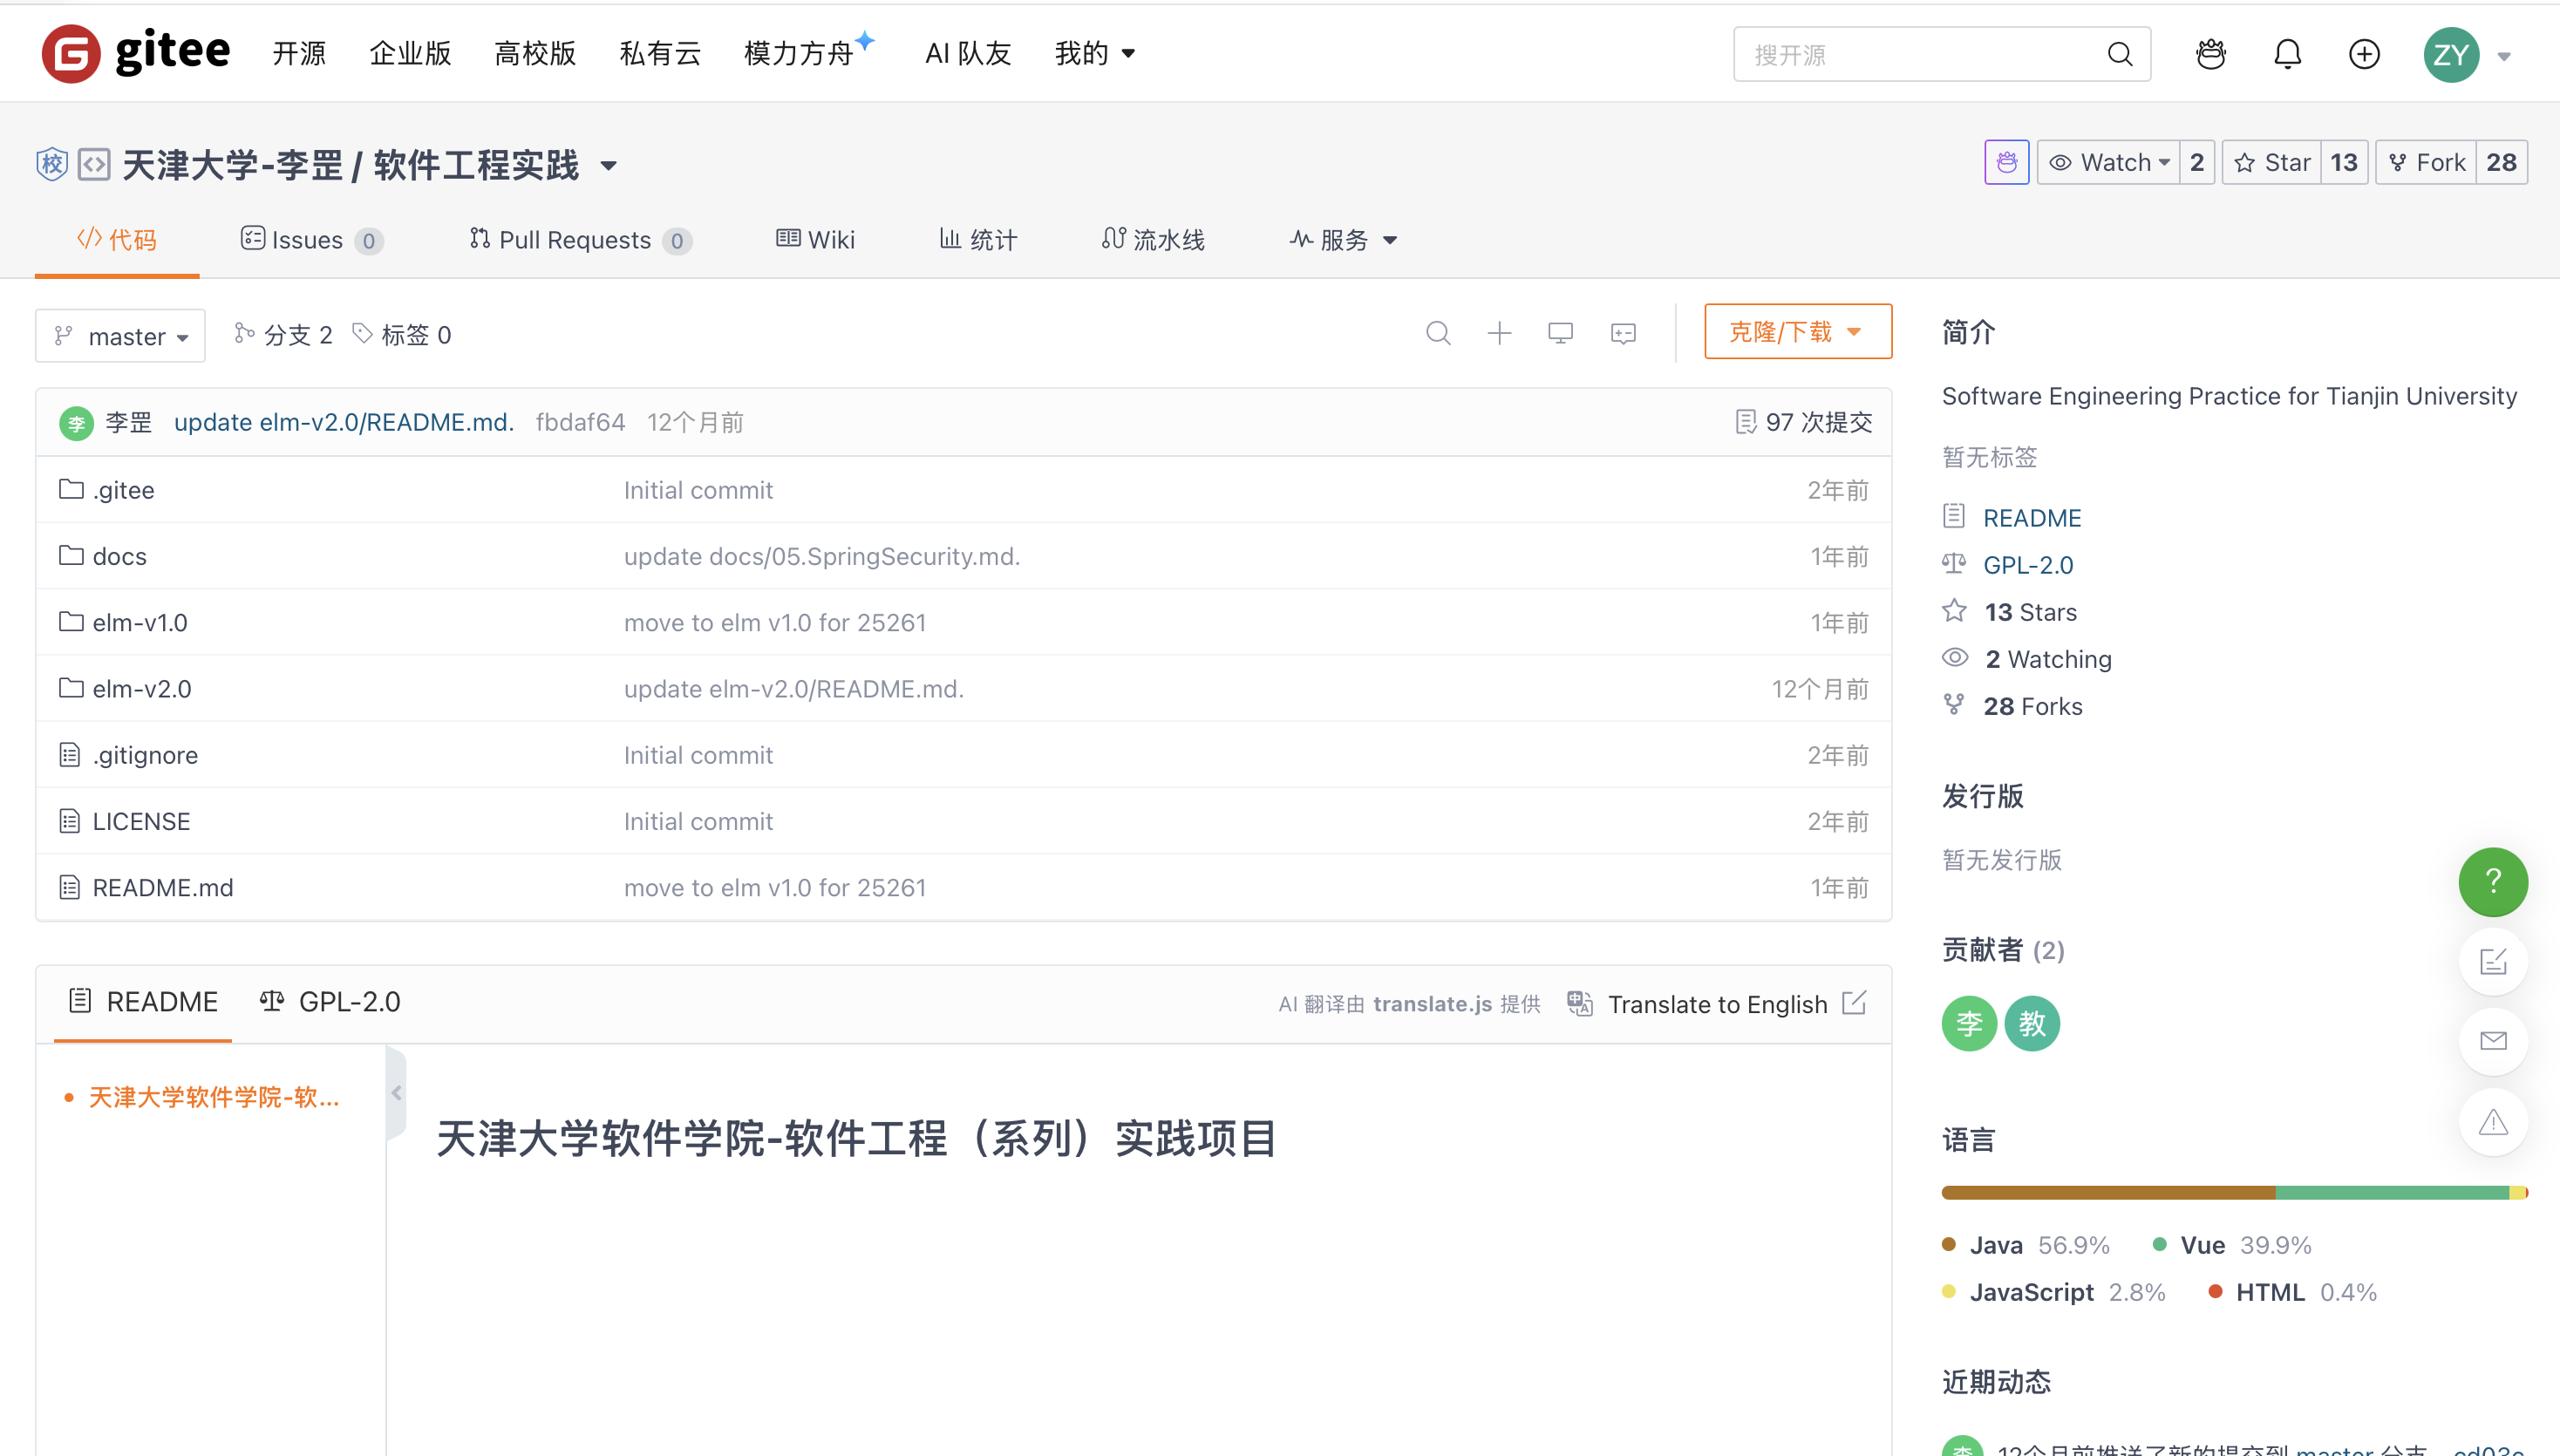
\includegraphics[width=.86\linewidth]{figures/report/process/course-repository.png}
  \caption{课程初始工程与仓库起点}
  \label{fig:process-course-repository}
\end{figure}
\section{开发阶段与可核对的产物}
项目过程不是先完成所有页面再集中拼接，而是在需求、基础框架、业务模块、整合验证和体验完善之间迭代。下表依据提交日期和提交内容整理阶段；阶段名称用于概括，不表示小组当时存在同名会议或正式里程碑审批。
\begin{longtable}{L{.19\linewidth}L{.28\linewidth}L{.44\linewidth}}
\caption{开发阶段与仓库证据}\\\toprule 时间&工作主题&可核对产物\\\midrule\endfirsthead\toprule 时间&工作主题&可核对产物\\\midrule\endhead
9 月 1--3 日&仓库建立与需求分析&\code{4fcbf00} 初始提交、\code{6e39d85} SRS 初版、\code{4d071aa} 需求修订，随后补充参与者、用例和页面结构图。\\
9 月 5--9 日&基础能力与业务模块并行&前后端基础、账号与权限、下单支付、商家商品、骑手配送等分支相继整合；\code{7c898f4} 合并 SRS 2.0，\code{39c5469} 合并骑手配送。\\
9 月 9 日&过程记录与回归&\code{21f7ec1} 补充测试输出，\code{d80eaba} 补充开发记录；保留结构契约检查和模块测试的不同证据口径。\\
9 月 11--14 日&AI 入口与界面完善&AI 点餐页面、分类商家列表、登录、订单页及交互动效逐步调整，多个界面分支通过合并提交整合。\\
9 月 15--16 日&全链路整合与交付整理&\code{e06d806} 合并 AI 界面并保留鉴权与结算保护；\code{06780ac}、\code{12c3d6e}、\code{d319c5e} 对返回导航补充测试、修复与重构；最终完善四端体验、部署和高德选址。\\\bottomrule
\end{longtable}
需求阶段的关键变化，是把“要做哪些功能”转化为“谁在什么条件下完成什么任务，失败时如何处理”。实现阶段则需要把订单金额、库存、身份与状态规则落实到服务端。最终阶段的界面完善不能替代回归检查：一个按钮或导航入口的修改，也可能影响登录态、订单确认和页面返回路径。

表中的日期来自仓库提交和产物形成时间，可以早于正式组会日期。以下叙述按照课程规定的关键节点补充开发过程，用于说明产物如何从需求分析逐步进入联调、验收和报告整理，不改变上表原有的仓库证据口径。

\subsection{分组与协作环境建立}
9月2日前后，小组完成成员确认、仓库访问检查和本地环境准备，并确定腾讯会议、微信群、飞书共享文档及 GitHub 的用途。成员先阅读课程要求和初始工程，再根据基础技术方向确定前端、后端、数据库和测试主责。此时形成的分工并不是后续工作的固定边界，而是用于保证每个关键方向都有明确责任人。

\subsection{需求分析与系统建模}
9月4日至8日，小组围绕四类角色、主要业务模块和完整履约流程撰写《软件需求规格说明书》。总体架构图用于说明系统参与者、前后端、数据库和外部服务之间的关系；UML 总用例图用于检查顾客、商家、骑手和管理员的职责是否覆盖。两类图共同把文字需求转换成可供开发和验收核对的结构。
\begin{figure}[H]
  \centering
  \begin{minipage}[t]{.54\linewidth}
    \centering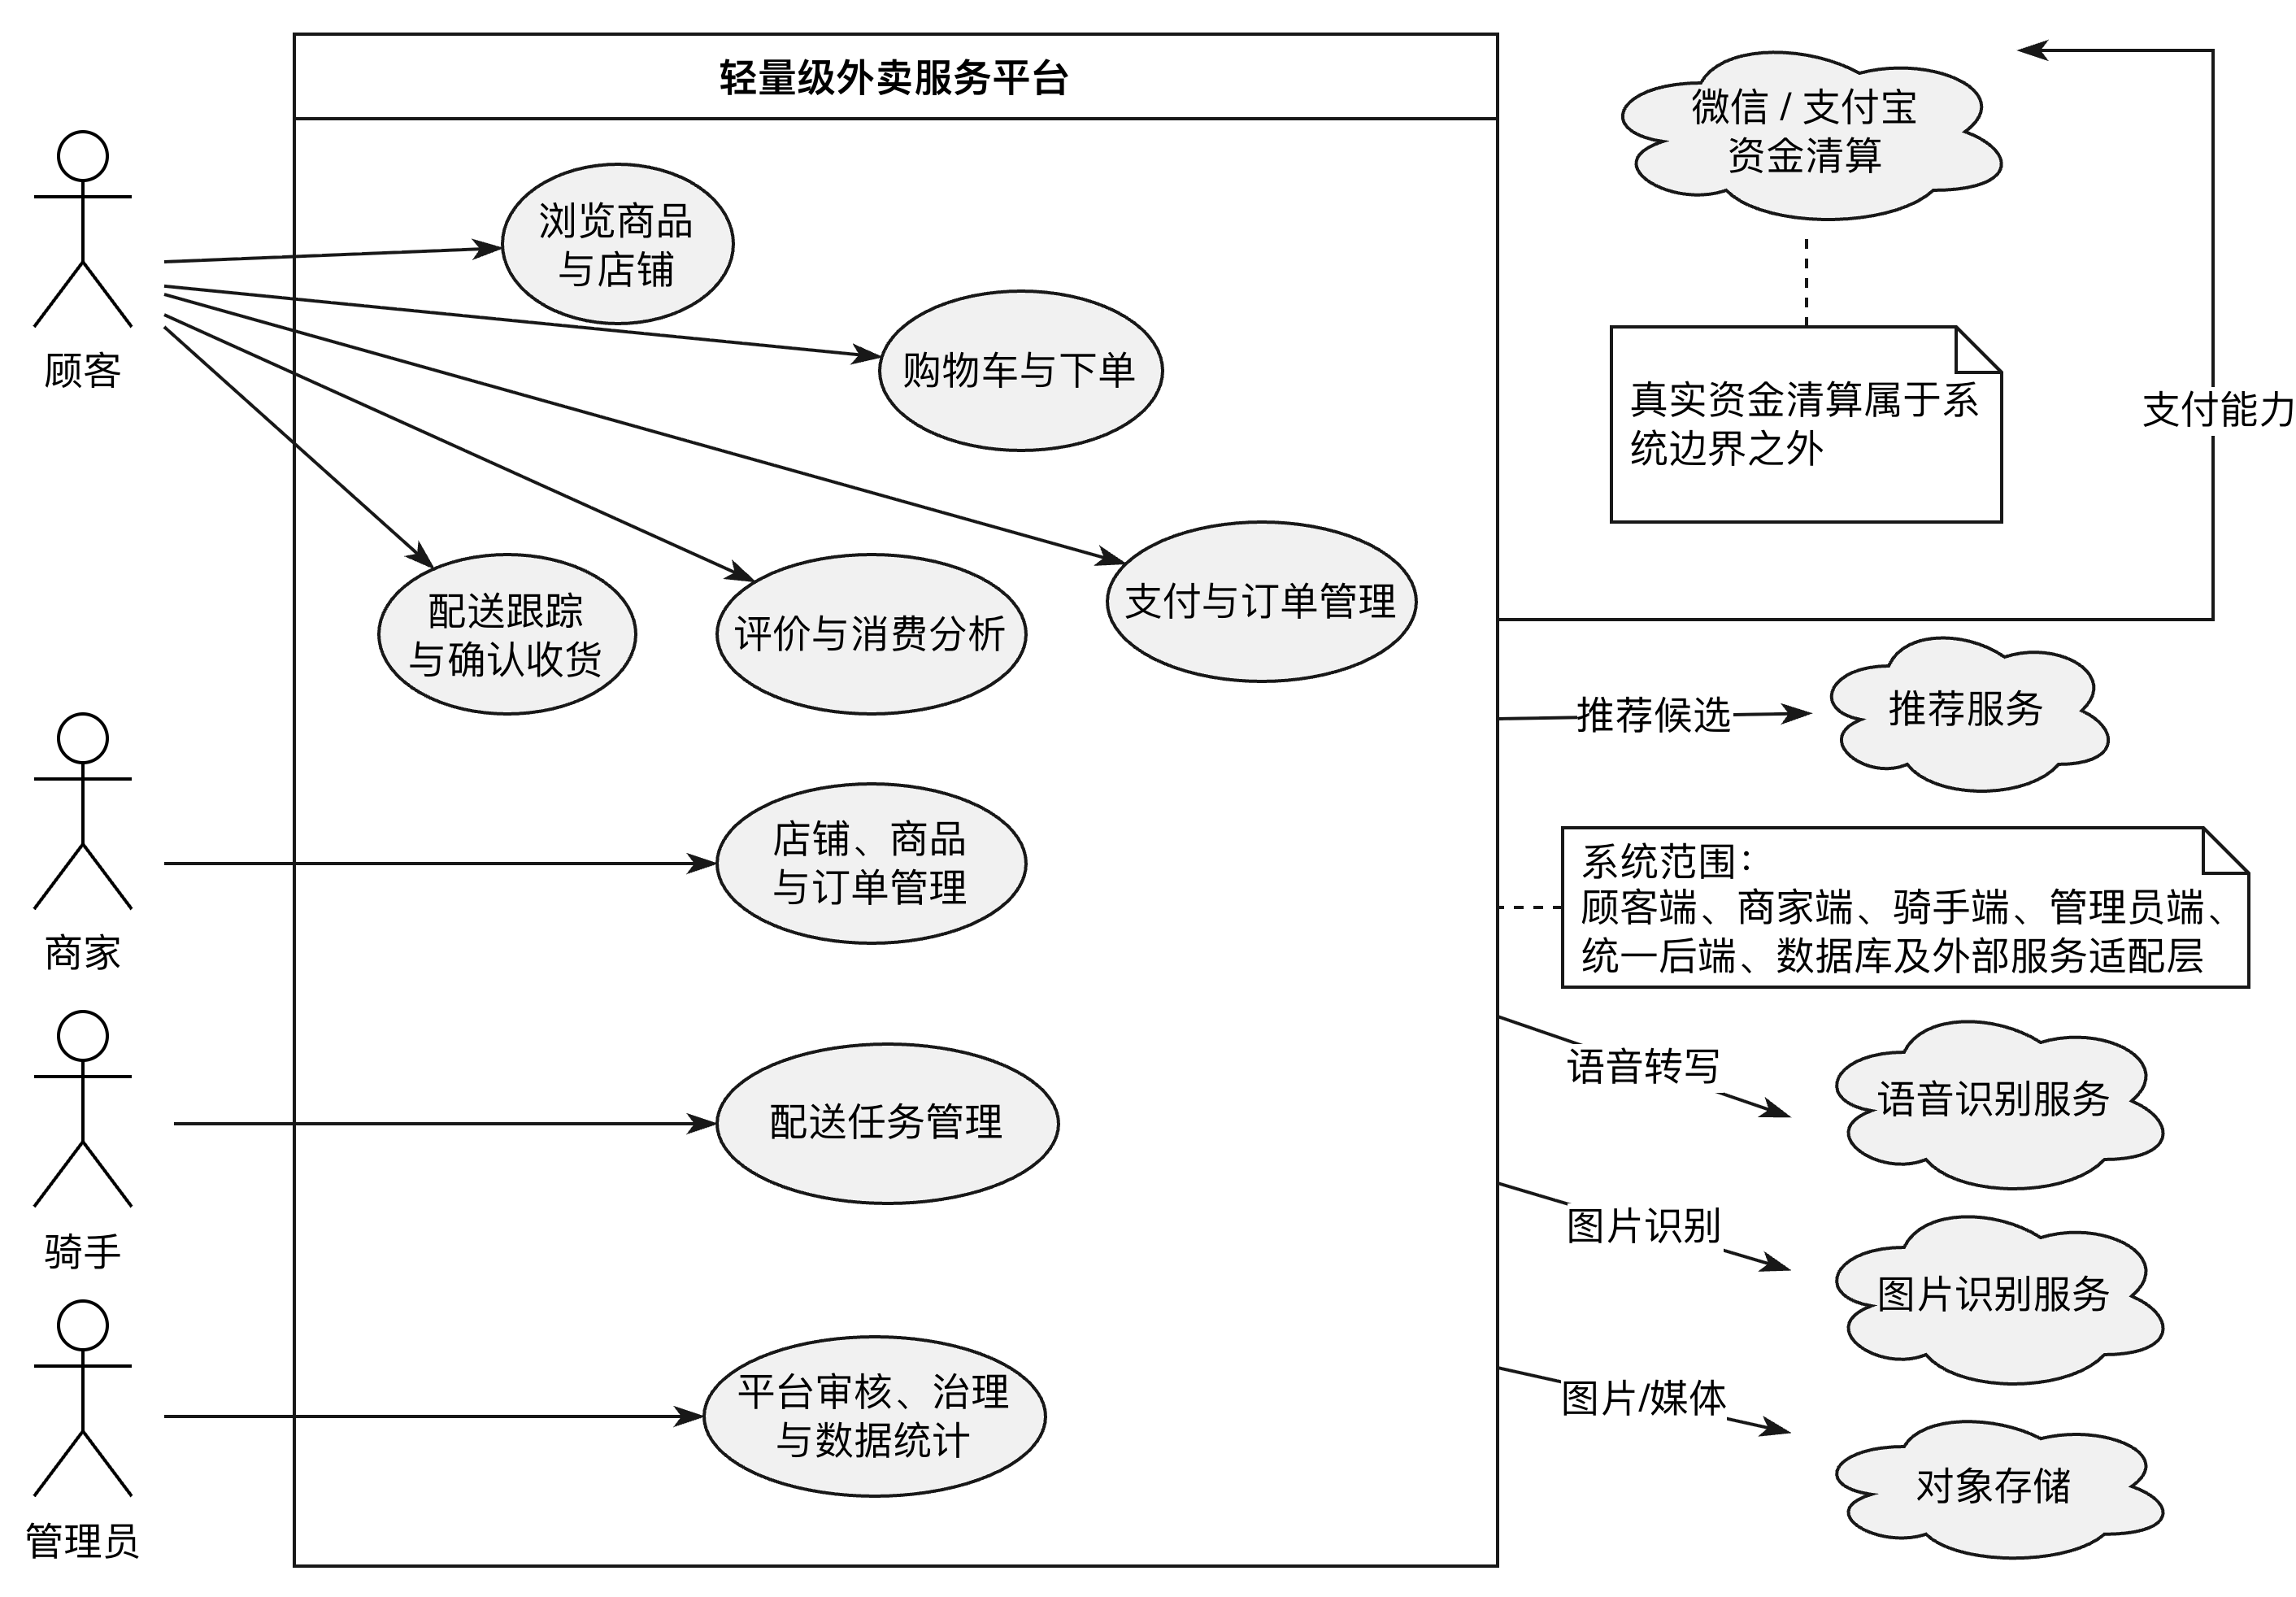
\includegraphics[width=\linewidth]{figures/report/process/architecture.png}\\[-2pt]
    \small（a）系统总体架构图
  \end{minipage}\hfill
  \begin{minipage}[t]{.40\linewidth}
    \centering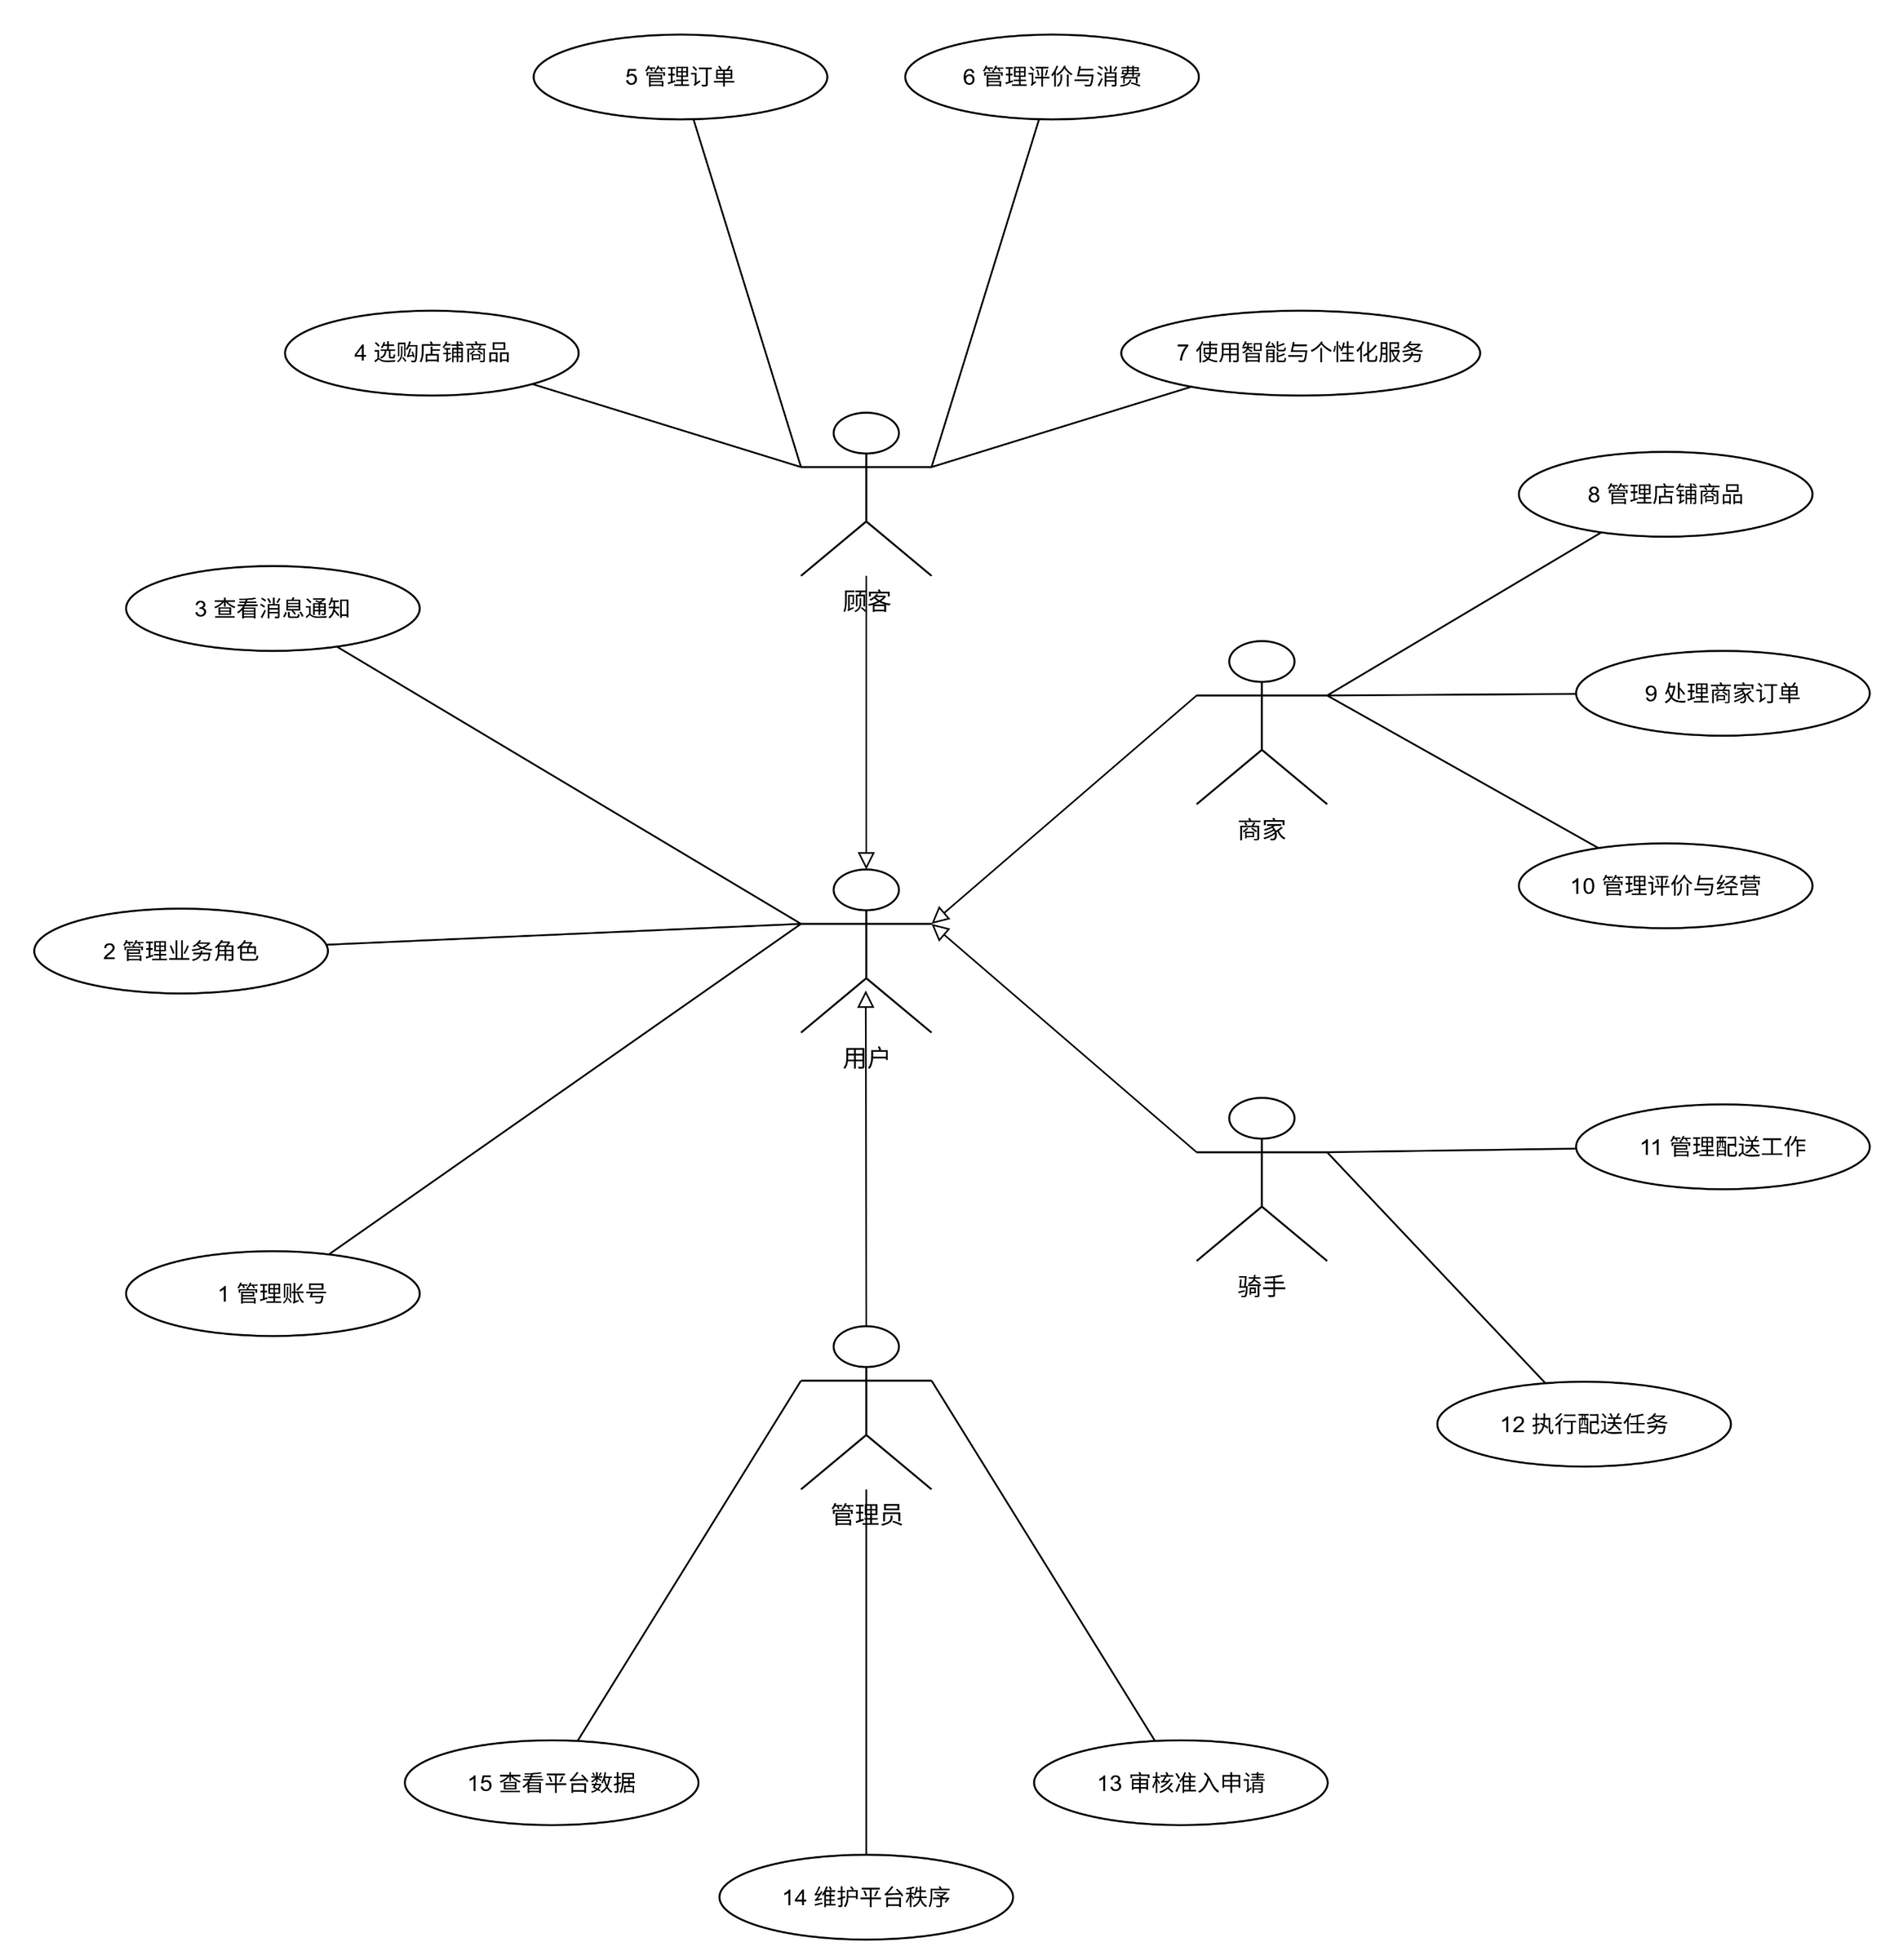
\includegraphics[width=\linewidth,height=.30\textheight,keepaspectratio]{figures/report/process/use-case.png}\\[-2pt]
    \small（b）UML 总用例图
  \end{minipage}
  \caption{需求分析阶段形成的系统模型}
  \label{fig:process-models}
\end{figure}

\subsection{阶段一开发与中期检查}
9月9日前后，小组按课程要求检查用户、商家、店铺、商品和订单等基础模块。检查不只关注页面是否存在，还核对请求参数、权限、状态变化和数据库支持。对未完成或前后端理解不一致的内容，小组重新形成任务清单；需求变化先确认业务规则及影响范围，再同步修改页面、接口、数据结构和测试检查项。

\subsection{分支开发与功能整合}
中期检查后，四名成员按照基础责任范围并行推进，同时围绕跨层业务开展联调。阶段性任务在独立分支完成，经过自测和 Pull Request 检查后进入主分支；出现冲突时，由涉及模块的成员共同核对，而不是仅以最后执行合并的人作为该功能的唯一贡献者。
\begin{figure}[H]
  \centering
  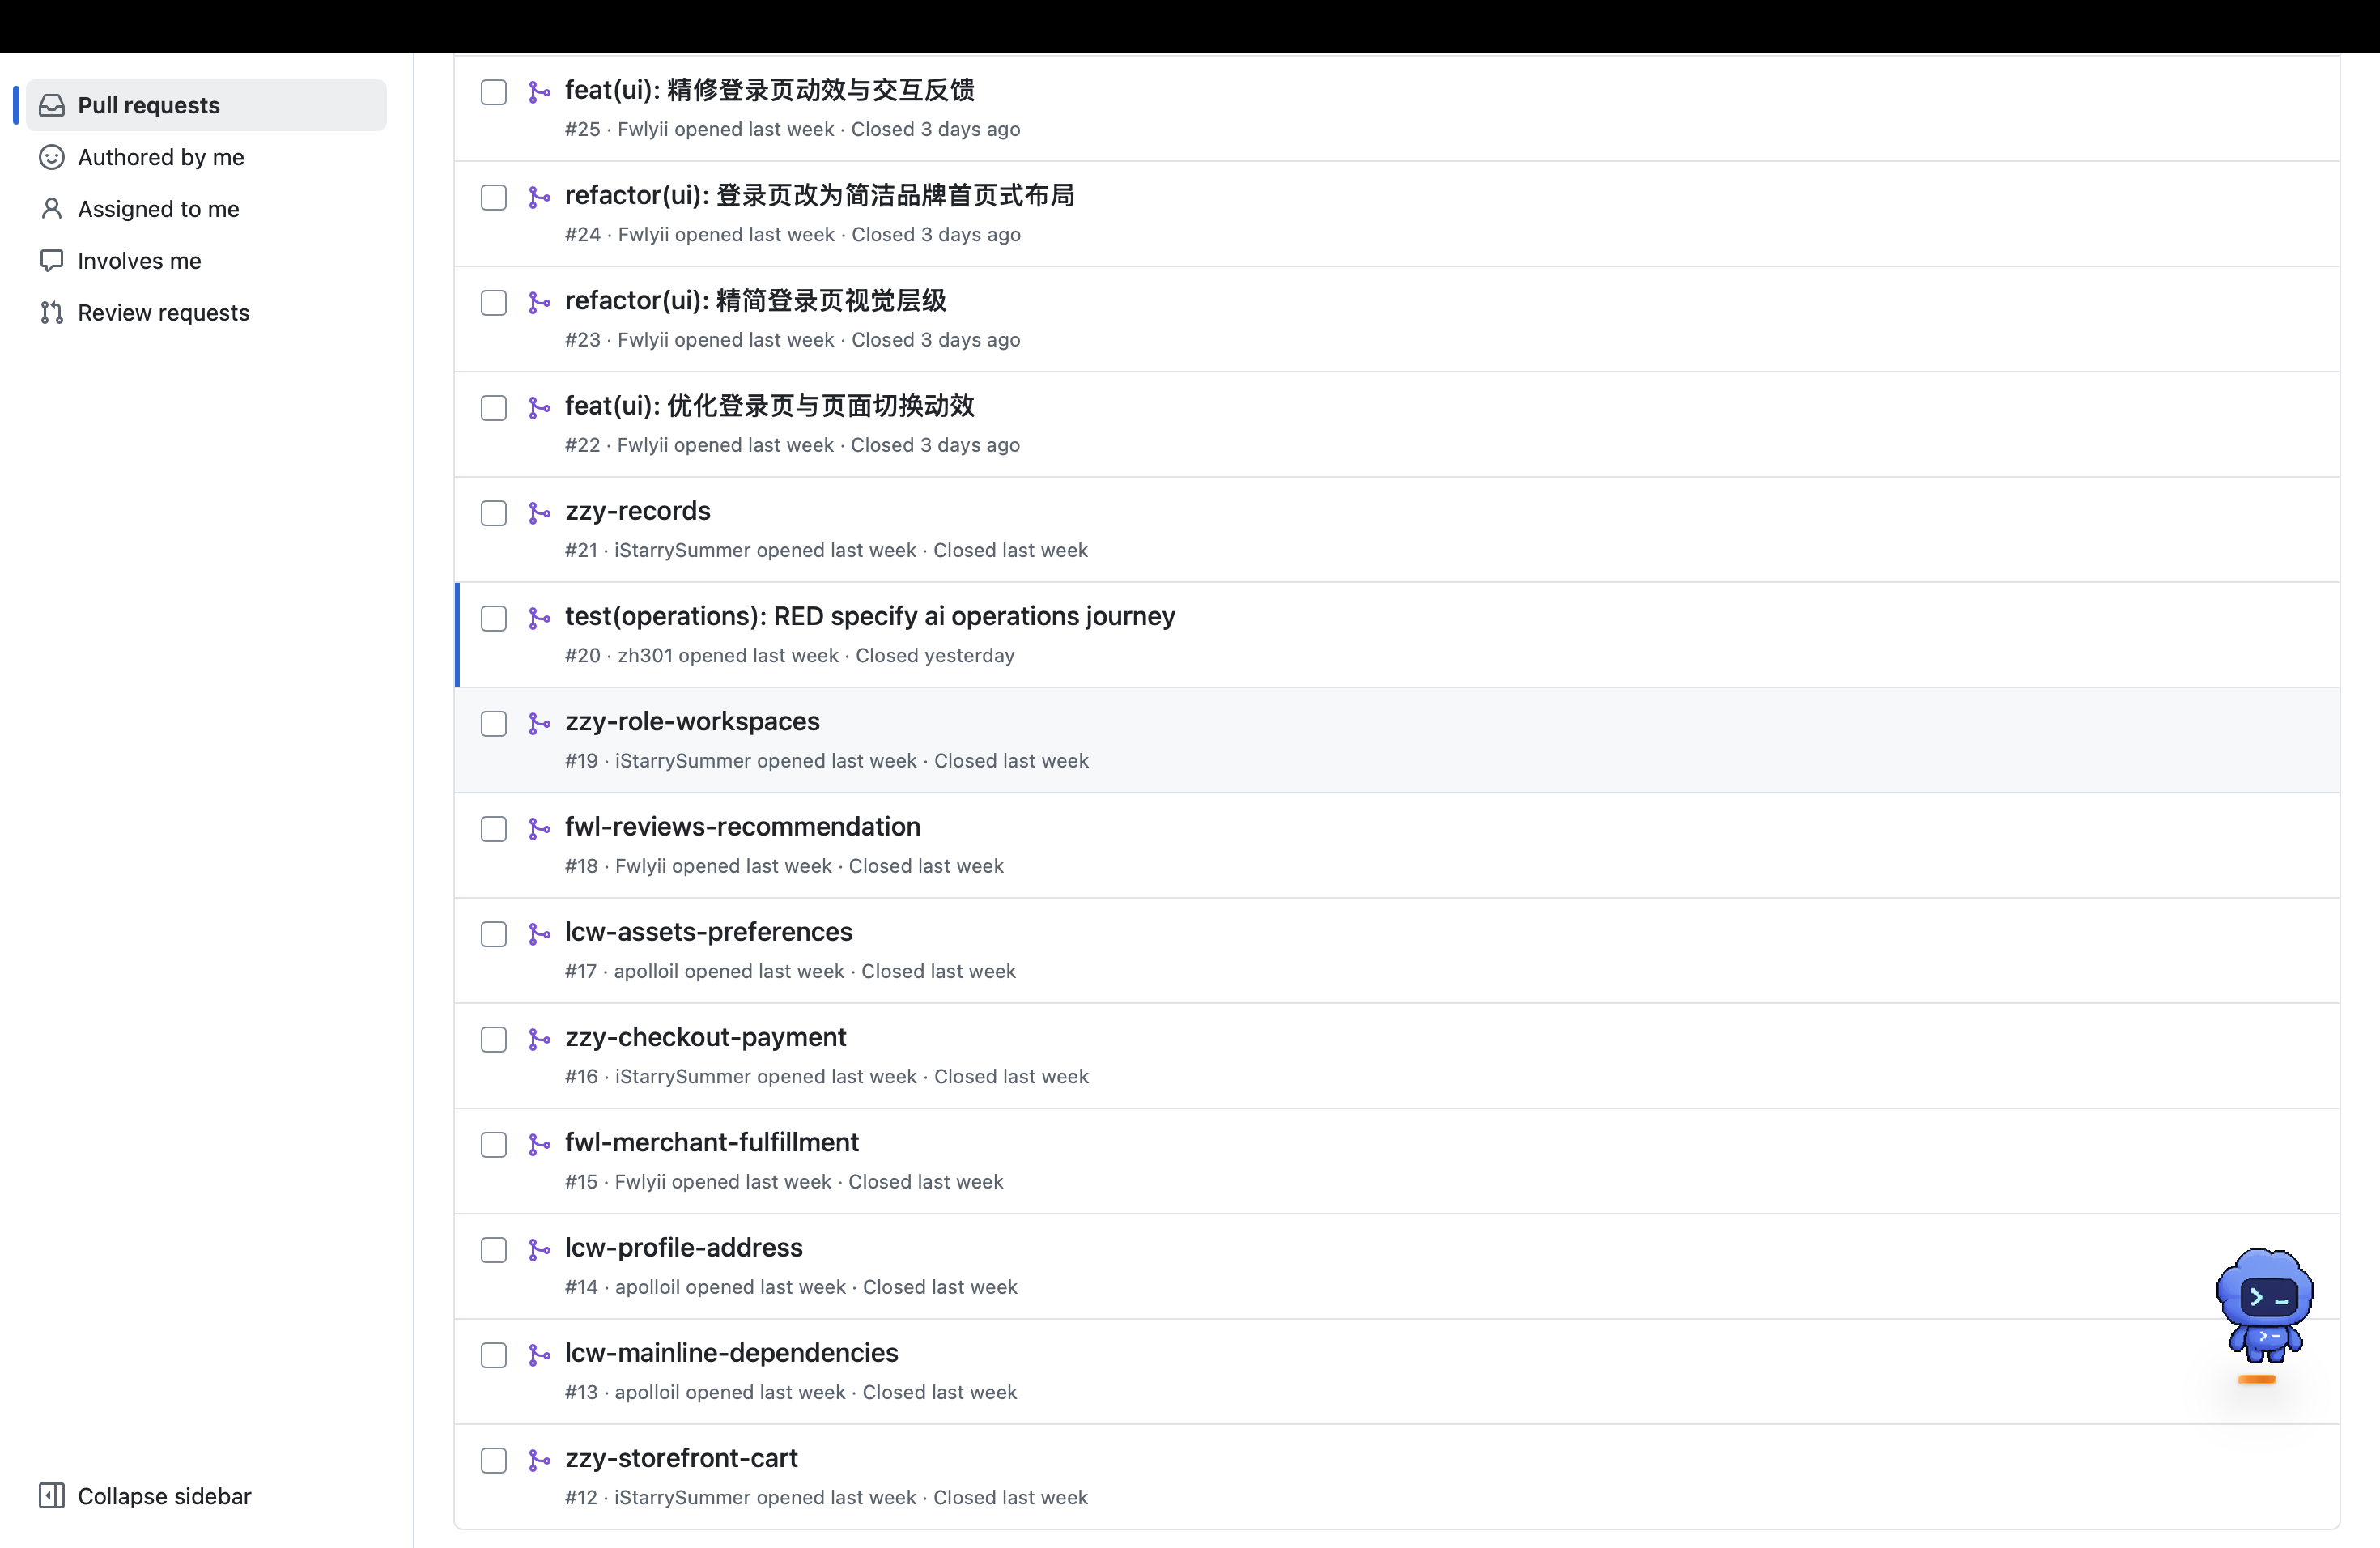
\includegraphics[width=.94\linewidth]{figures/report/process/pull-requests.png}
  \caption{功能分支通过 Pull Request 合并的记录}
  \label{fig:process-pull-requests}
\end{figure}

9月15日前后，小组将顾客端、商家端、骑手端和管理端整合到同一测试版本，检查角色入口、权限、路由及主要业务链路。四端界面合并图用于说明阶段成果已经从单独页面进入统一运行环境；它只表示界面与入口的整合情况，具体业务正确性仍由接口测试和回归测试确认。
\begin{figure}[H]
  \centering
  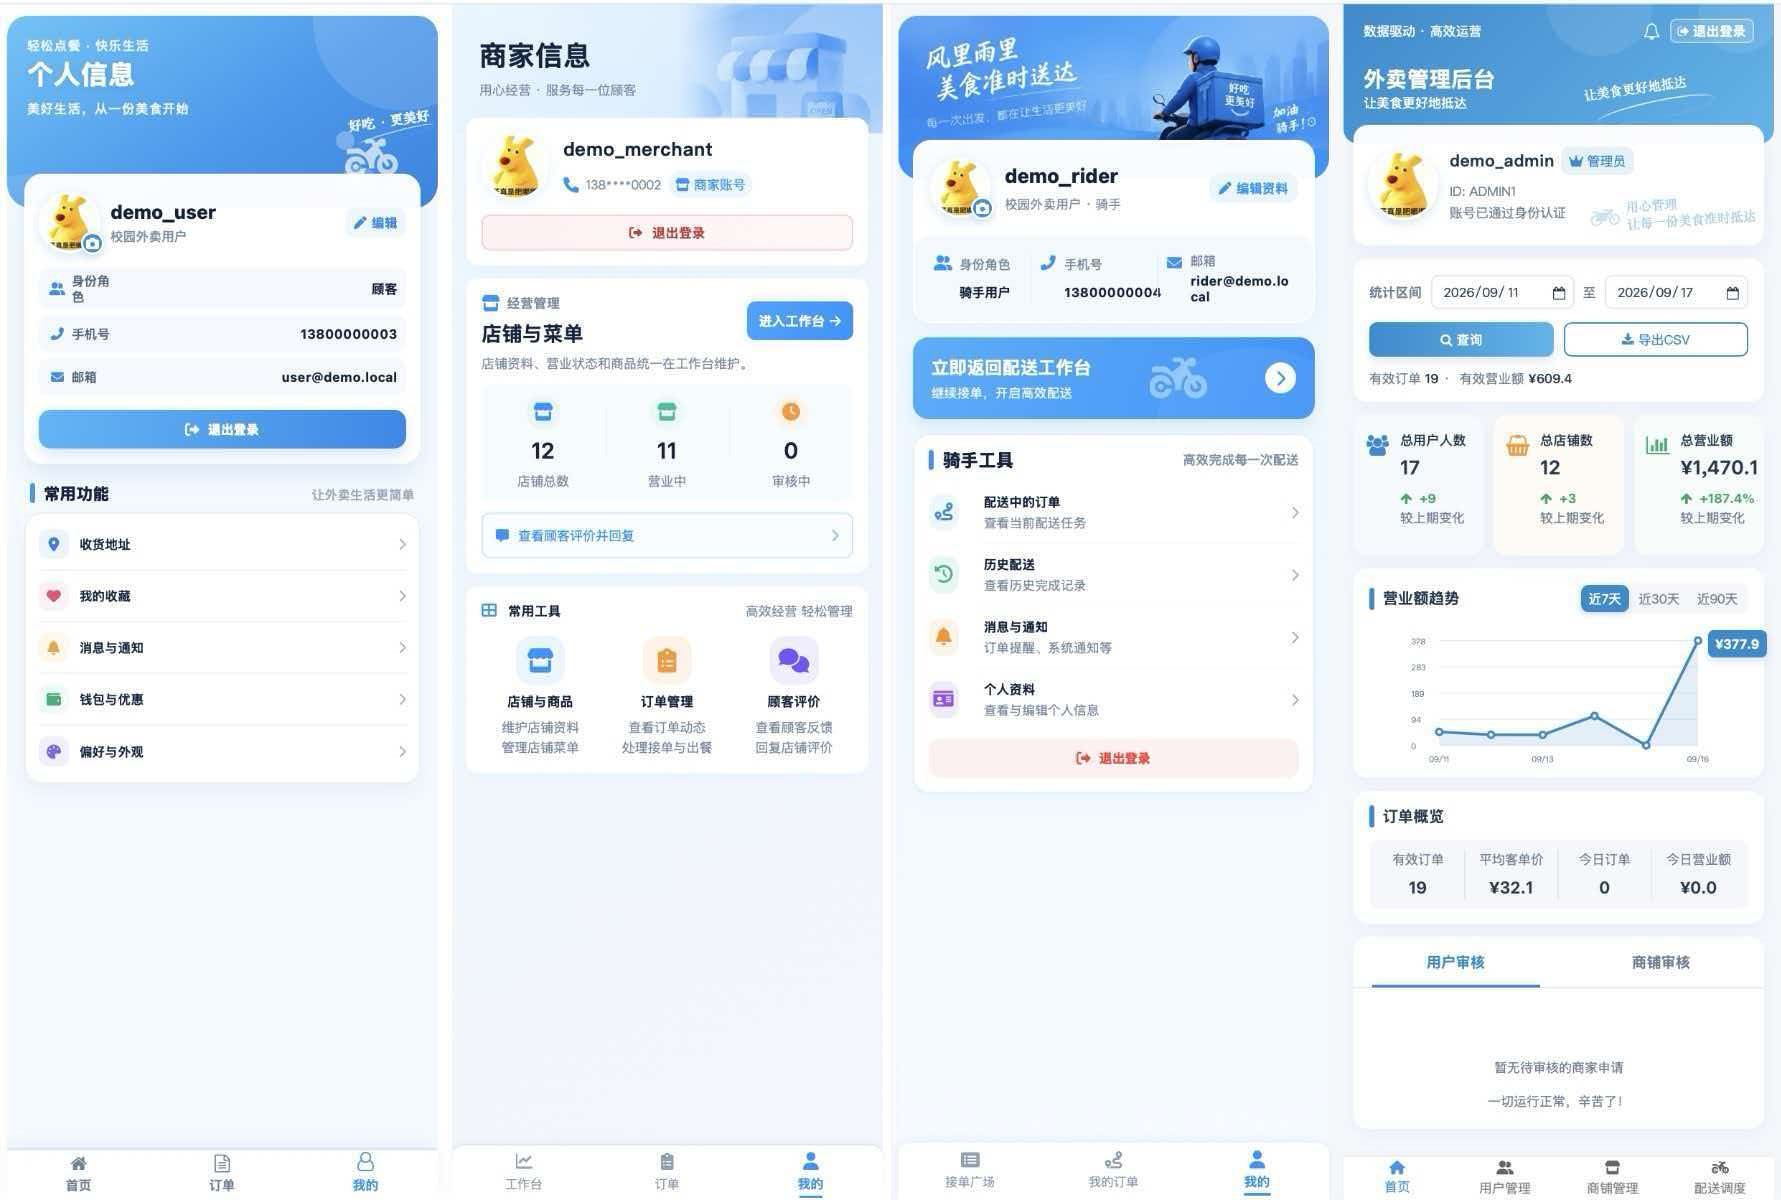
\includegraphics[width=.88\linewidth]{figures/report/process/four-roles.jpg}
  \caption{顾客端、商家端、骑手端和管理端的整合结果}
  \label{fig:process-four-roles}
\end{figure}

\subsection{交叉验收、课程验收与报告整理}
在交叉验收前，小组已经通过自动化测试和人工功能筛查检查本组项目，并使用统一缺陷表记录人工发现的问题，具体方法见项目测试章节。9月16日的交叉验收是本组依据其他小组提交的需求文档和可运行版本，对其他小组的成果进行检查；这一过程与本组内部缺陷筛查是两类不同活动，不能使用本组缺陷登记表代替交叉验收记录。

9月18日由教师对本组项目进行课程验收。9月19日以后，小组结合课程验收意见继续修正本组问题，并开始收集需求、设计、实现、测试和协作证据。报告整理不是重新构造开发过程，而是把仓库、共享文档、会议记录、缺陷表和运行截图相互核对，使文字结论能够追溯到相应产物。
\section{组会与协作方式}
项目开发初期，小组主要通过腾讯会议、即时通信和共享文档开展协作，但没有在每次会议结束后立即形成统一格式的书面纪要。报告整理阶段，小组依据课程时间节点、腾讯会议历史、即时通信内容、共享文档、代码提交与合并记录以及组员回忆，对九次线上会议进行了补充整理。因此，以下内容是对实际协作过程的事后整理，并非会议录音的逐字转写。仓库提交日期用于核对开发产物，不直接等同于组会日期；腾讯会议历史截图也仅用于说明线上会议工具的使用情况，不单独证明每次会议的全部议题和出席情况。

协作接口主要包括：前端与后端确认请求和错误反馈，后端与数据库核对事务与历史快照，AI 与商品数据模块核对推荐依据，测试与地图模块验证定位失败和多角色履约。上述依赖来自项目实现和分工；具体会议内容以小组补充整理并共同确认的记录为依据。

\subsection{前八次线上会议}
\subsubsection{第一次线上会议（9月1日）：分组、仓库与协作方式}
\begin{enumerate}
  \item 根据课程安排确定项目小组由范文丽、李承文、赵紫怡和仲禹潼四名成员组成，并确认项目仓库地址及成员访问权限。
  \item 确定腾讯会议、微信群、飞书共享文档和 GitHub 的用途；普通文档保存在仓库 \code{docs} 目录，外部共享文档地址记录在根目录 \code{README.md} 中。
  \item 确定基础责任范围：范文丽主责前端与看板，李承文主责后端与红包积分，赵紫怡主责数据库与 AI，仲禹潼主责测试与高德地图。
  \item 约定基础分工不等于独立开发，需求核对、接口联调、缺陷修复和报告整理由全组共同参与。
\end{enumerate}

\subsubsection{第二次线上会议（9月3日）：需求确定与需求文档}
\begin{enumerate}
  \item 结合课程初始工程和课程要求，讨论顾客端、商家端、骑手端和管理端的建设范围。
  \item 梳理用户管理、商家管理、店铺管理、商品管理、购物车、订单管理、配送和后台管理等核心模块。
  \item 明确《软件需求规格说明书》的主体结构，包括项目背景、业务概念、功能性需求、非功能性需求、系统角色、用例模型和主要业务流程。
  \item 要求需求描述、业务流程、UML 图和后续代码实现相互对应；新增设想只有在明确业务规则和影响范围后才进入开发任务。
\end{enumerate}

\subsubsection{第三次线上会议（9月6日）：需求复核与系统建模}
\begin{enumerate}
  \item 汇报需求文档的整理进度，集中检查不同成员撰写内容之间的术语、角色和功能边界。
  \item 讨论系统总体架构图和 UML 总用例图，核对四类角色与各功能模块之间的关系。
  \item 梳理用户、店铺、商品、订单、地址、收藏、评价、钱包和积分等核心业务对象及其关联。
  \item 确认阶段一优先完成基础业务功能，个性化、可视化和智能化内容在基础流程稳定后继续完善。
  \item 约定阶段性任务使用独立分支，功能完成并自测后通过 Pull Request 合并。
\end{enumerate}

\subsubsection{第四次线上会议（9月8日）：中期检查与任务调整}
\begin{enumerate}
  \item 按课程中期检查要求，检查用户管理、商家管理、店铺管理、商品管理和订单管理等阶段一功能。
  \item 对尚未完成、前后端不一致或暂时无法正常运行的功能建立任务清单，并按问题所属模块重新分配工作。
  \item 范文丽继续完善四端页面、导航结构和数据看板；李承文继续完善订单业务与资产功能；赵紫怡继续完善数据库结构和 AI 调用；仲禹潼继续整理测试检查项并推进地图功能。
  \item 明确中期检查后进入功能补全和集中联调阶段；需求变化需要同时检查页面、接口、数据结构和测试用例。
\end{enumerate}

\subsubsection{第五次线上会议（9月10日）：分支合并与功能补充}
\begin{enumerate}
  \item 汇报中期检查后各模块的修改进度，通过 Pull Request 合并已经完成的阶段性功能。
  \item 集中处理代码冲突、依赖关系和配置差异，核对前端请求、后端接口、数据库字段和返回数据结构。
  \item 讨论四端整合方式，要求顾客端、商家端、骑手端和管理端使用统一后端服务并遵守角色权限。
  \item 确认继续完善用户偏好、钱包积分、红包、数据看板、AI 辅助交互和地图服务等扩展内容。
  \item 要求各成员在合并前完成基本自测，并在 Pull Request 中说明主要修改和验证情况。
\end{enumerate}

\subsubsection{第六次线上会议（9月12日）：第一次集中联调}
\begin{enumerate}
  \item 开展集中前后端联调，检查登录、店铺浏览、商品查看、购物车、订单提交、订单处理和后台管理等流程。
  \item 范文丽重点处理页面布局、导航和数据展示；李承文重点处理订单及资产业务；赵紫怡重点处理数据库关联和 AI 服务调用；仲禹潼重点执行功能、边界及地图测试。
  \item 建立统一缺陷登记表，记录问题类型、所属模块、问题描述、复现步骤、截图、修改建议和处理状态。
  \item 约定缺陷修复后重新执行相关业务链路，避免仅验证发生错误的单个页面或接口。
\end{enumerate}

\subsubsection{第七次线上会议（9月15日）：开发完成与测试版本}
\begin{enumerate}
  \item 按课程节点检查全部开发任务，将工作重点由功能扩展转向整合、测试和交付。
  \item 合并成员分支，处理冲突、接口差异和配置问题，检查四端入口、角色权限与页面跳转。
  \item 检查用户操作、店铺与商品管理、购物车、订单生成、订单状态变化和后台管理等主要业务链路。
  \item 检查钱包积分、数据看板、AI 辅助交互和地图服务等特色内容是否具备测试条件。
  \item 生成用于交叉验收的可部署测试版本，并核对《软件需求规格说明书》与当前实现是否一致。
  \item 原则上不再扩大功能范围，后续集中处理交叉验收、缺陷修复和展示准备。
\end{enumerate}

\subsubsection{第八次线上会议（9月16日）：交叉验收总结与课程验收准备}
\begin{enumerate}
  \item 汇总本组在9月16日验收其他小组成果时形成的检查记录，依据对方需求文档核对功能完成情况、业务流程和运行表现。
  \item 将交叉验收意见按需求符合性、功能表现、交互问题和测试证据进行整理，不把其他小组的问题登记为本组项目缺陷。
  \item 继续检查本组项目，准备9月18日课程验收所需的账号、店铺、商品、订单和统计数据，并检查展示环境和备用方案。
  \item 范文丽检查页面、导航和看板；李承文检查后端业务及钱包积分；赵紫怡检查数据库、AI 与异常降级；仲禹潼组织复测并检查地图功能。
  \item 讨论最终展示顺序并进行模拟展示，确认9月18日全组参加课程验收和问题回答。
\end{enumerate}

\subsection{第九次线上会议（9月19日）：验收复盘与报告安排}
\begin{enumerate}
  \item 复盘9月18日课程验收，整理展示过程中被指出的问题和需要进一步完善的内容。
  \item 将业务问题、页面细节和运行稳定性问题补充到缺陷登记表，按成员责任范围安排修复和复测。
  \item 修改完成后重新执行核心业务流程，检查修复内容是否影响其他模块。
  \item 讨论实验报告结构，确定需要整理需求分析、系统设计、项目实现、测试、成员分工、开发过程、AI 使用情况和问题反思。
  \item 收集系统架构图、UML 图、Pull Request、贡献统计、会议记录、共享文档、缺陷登记和四端运行截图等材料。
  \item 明确报告事实应以代码仓库、现有文档和可核对截图为依据，讨论过但没有实现的设想不写成最终成果。
  \item 安排9月27日前完成报告撰写、交叉检查、LaTeX 编译和最终提交。
\end{enumerate}

\begin{figure}[H]
  \centering
  \begin{minipage}[t]{.36\linewidth}
    \centering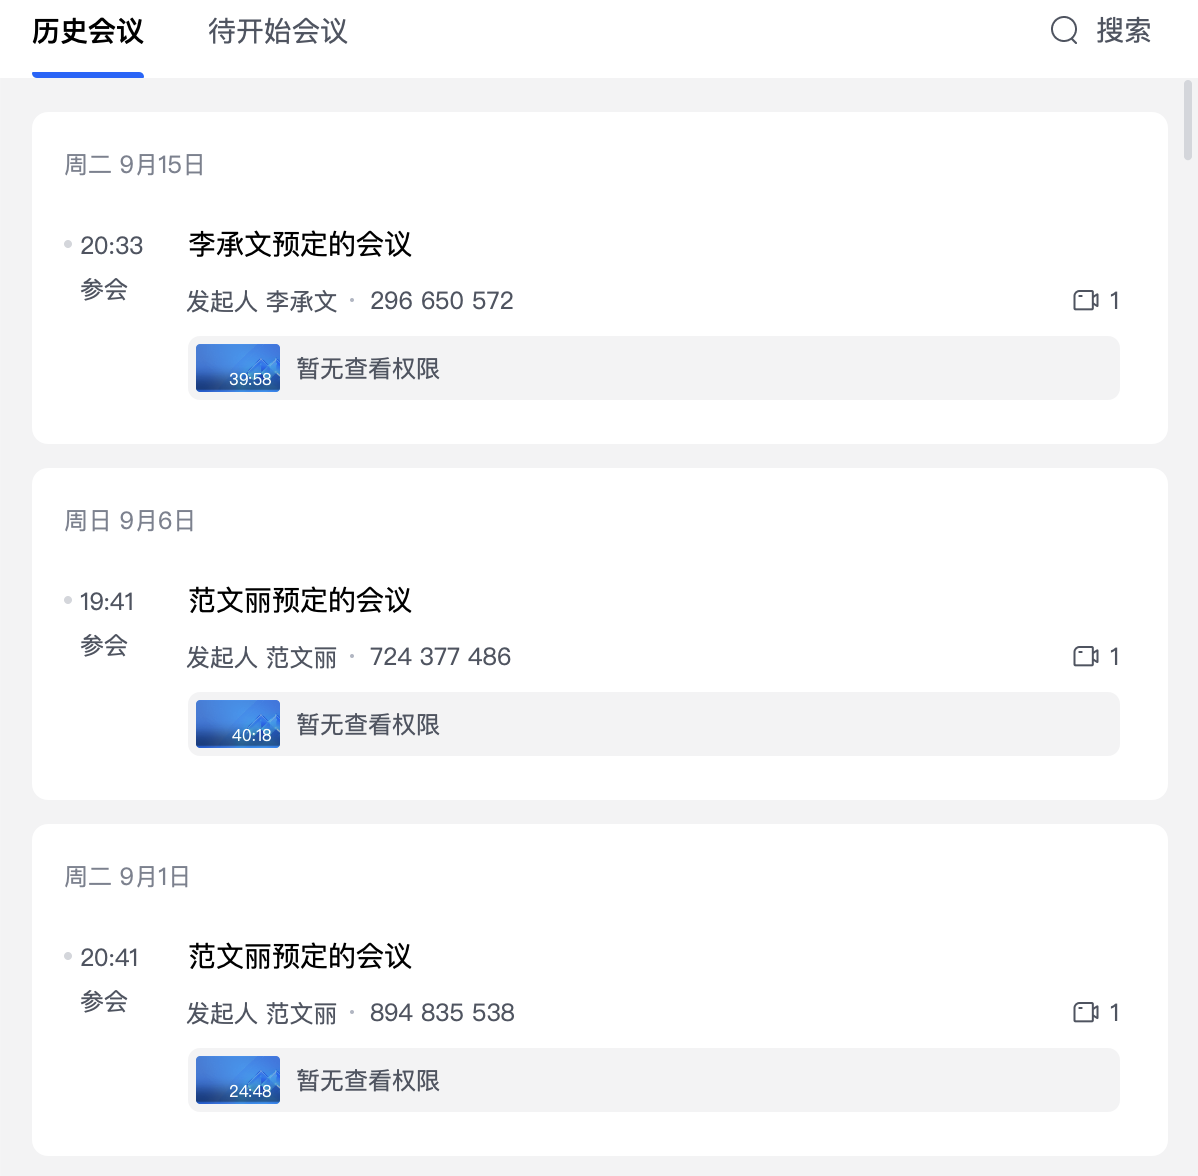
\includegraphics[width=\linewidth]{figures/report/process/meeting-history.png}\\[-2pt]
    \small（a）腾讯会议历史页面
  \end{minipage}\hfill
  \begin{minipage}[t]{.60\linewidth}
    \centering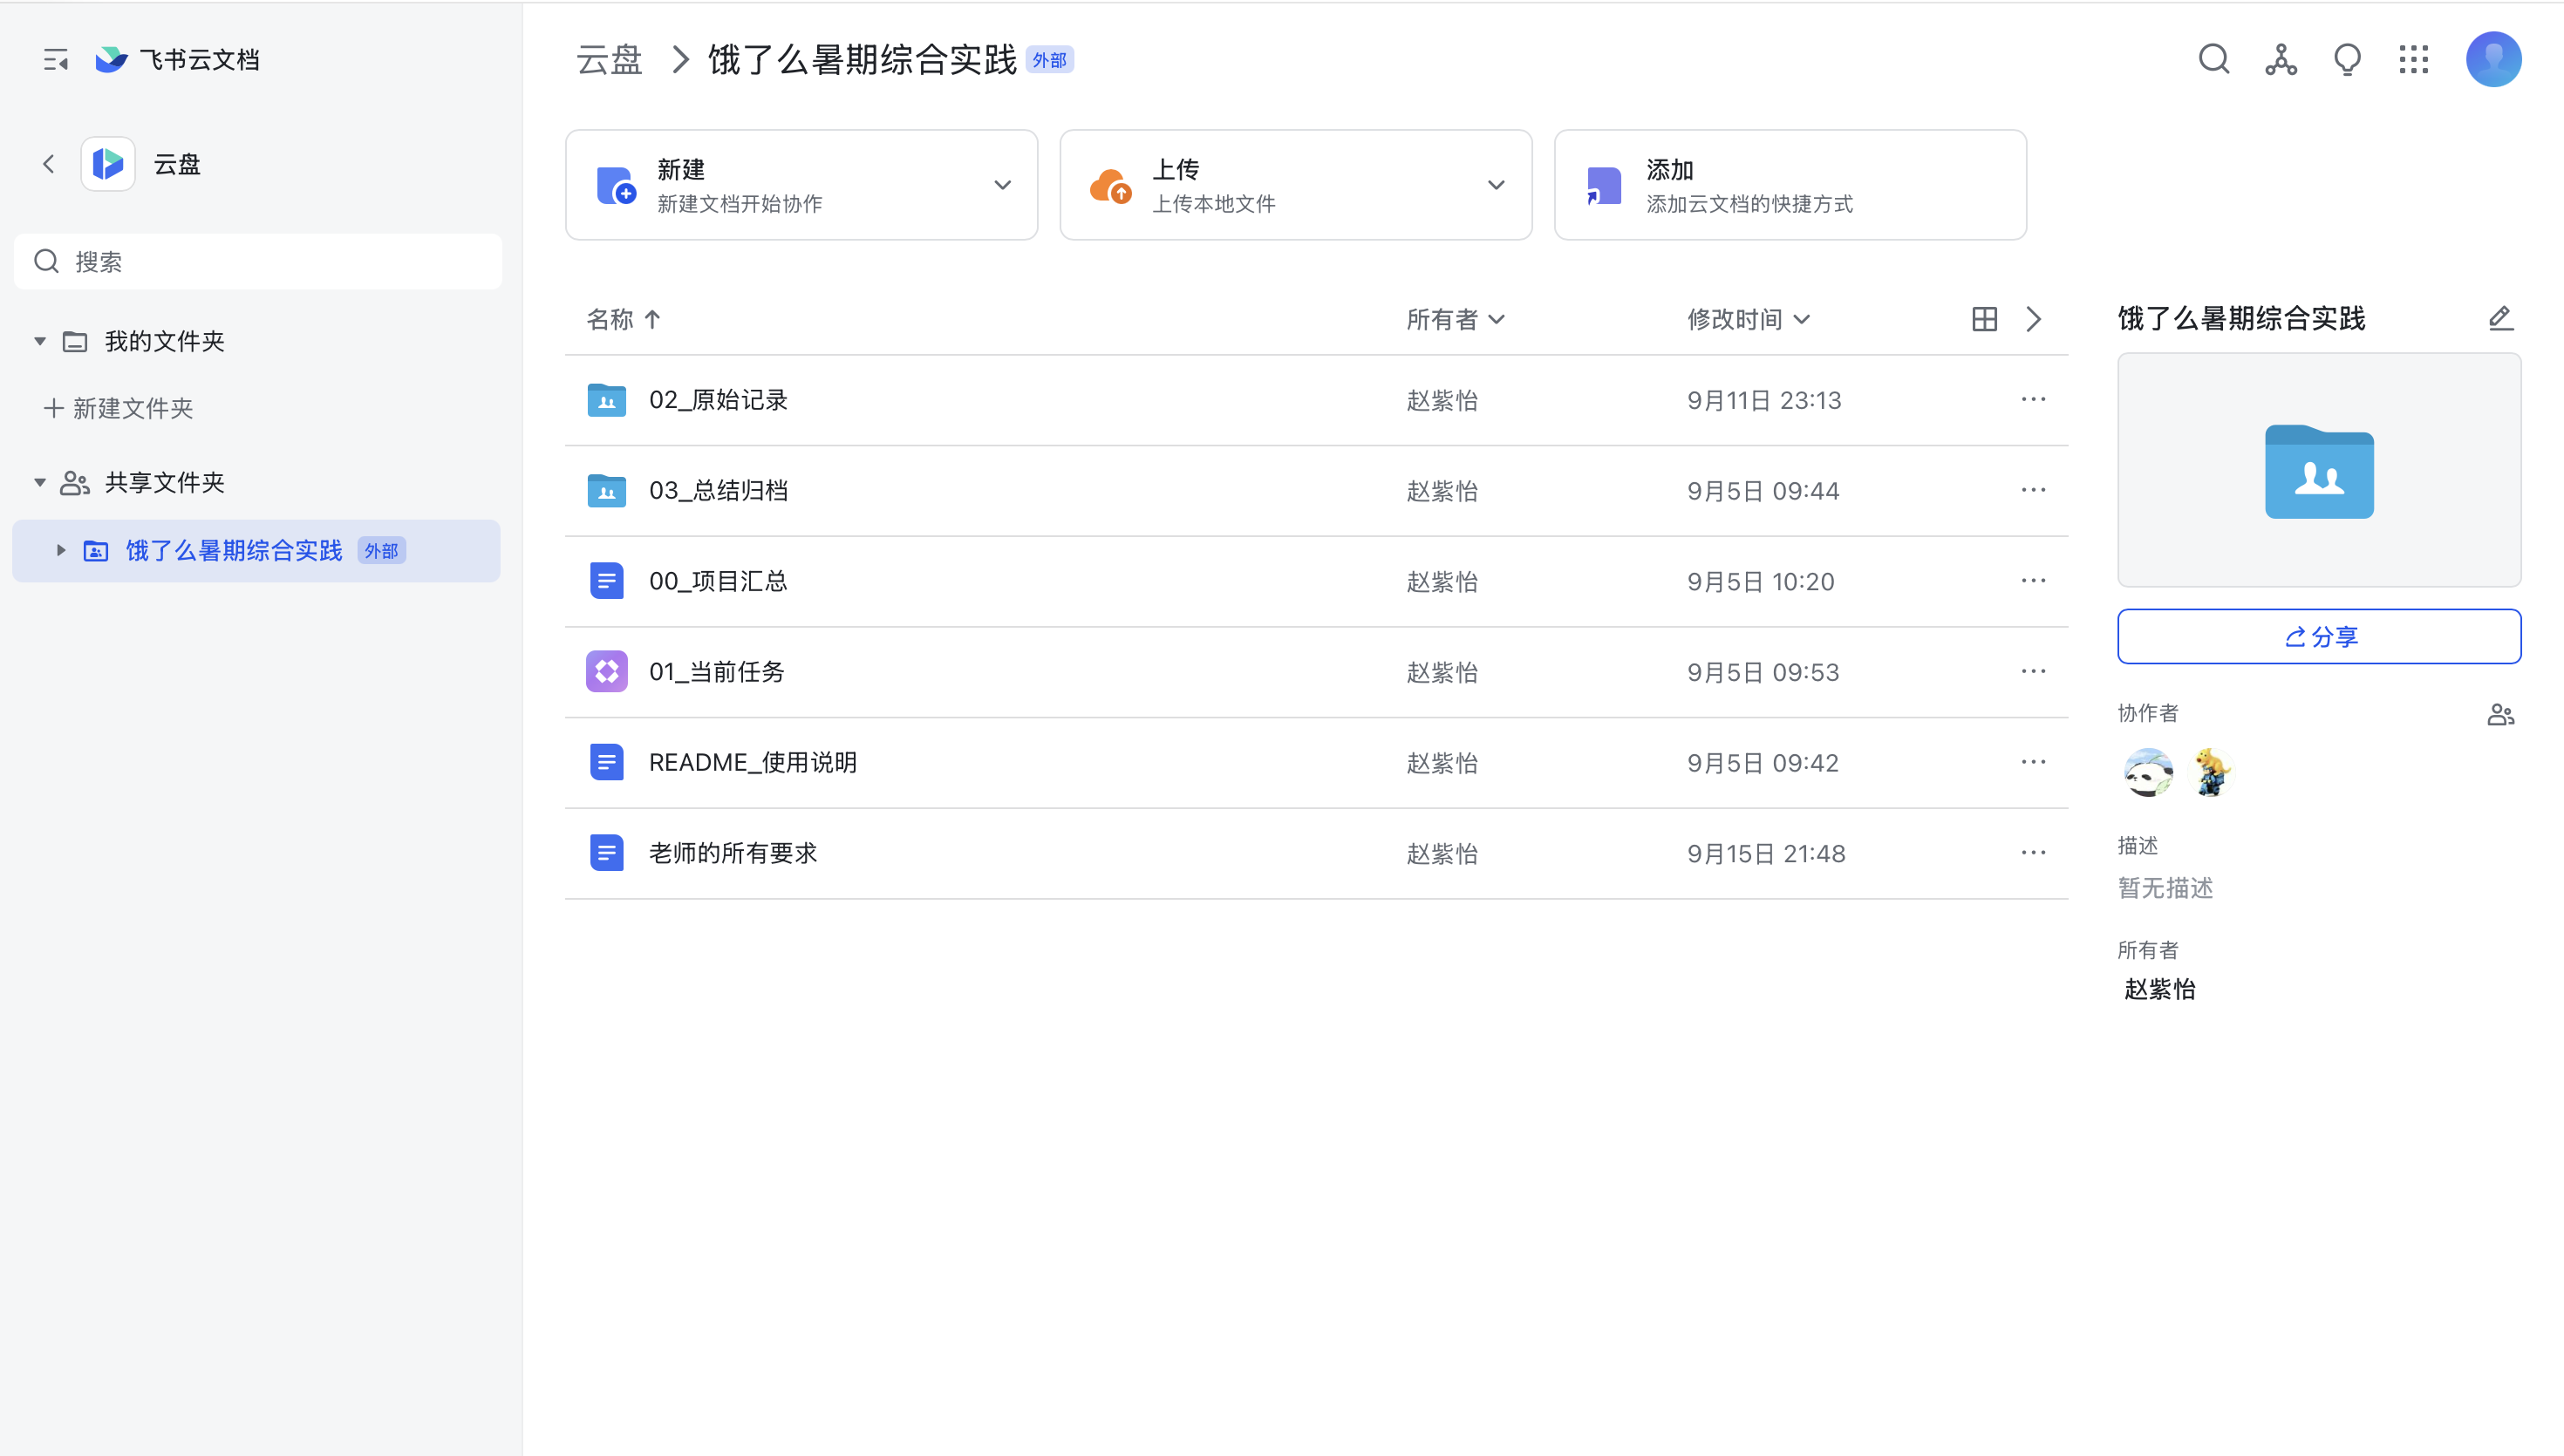
\includegraphics[width=\linewidth]{figures/report/process/feishu-workspace.png}\\[-2pt]
    \small（b）飞书共享文档空间
  \end{minipage}
  \caption{线上会议与共享文档协作工具}
  \label{fig:process-collaboration-tools}
\end{figure}

飞书讨论中还记录了阶段任务使用独立分支、完成后合并到主分支以及及时清理无用分支等协作约定。这类即时讨论用于补充正式会议后的执行细节，但聊天中提出的设想只有在仓库或运行结果中得到验证后，才作为已实现事实写入报告。
\begin{figure}[H]
  \centering
  
\includegraphics[width=.90\linewidth]{figures/report/process/branch-discussion.png}
  \caption{飞书中关于分支开发与合并方式的讨论记录}
  \label{fig:process-branch-discussion}
\end{figure}
\section{CheckIn 与 CheckOut 的统计口径}
本报告将 CheckIn 具体统计为 Git 提交：所有远端分支可达提交去重后共 265 条，包含 38 条合并提交，普通提交 227 条；其中 \code{main} 可达 258 条。统计按提交对象去重，不把同一提交在多个分支出现重复计数；日期使用作者日期。两个不同邮箱的 Chengwen，以及同邮箱的 mao/iStarrySummer、Zhong Yutong/Zita 分别按作者身份组归并。个人实名与账号关系以成员确认表为准。

CheckOut 通常指本地切换或检出分支。远端提交历史不保存每位成员的 checkout、fetch、pull 或 clone 次数，因此不能给出这些行为的实际频率，也不能把某天没有提交等同于当天没有工作。提交次数不是贡献度评分：文档、测试、界面细分提交、合并提交和一次集中导入所代表的工作量并不相同。
\begin{longtable}{L{.30\linewidth}C{.12\linewidth}C{.14\linewidth}C{.12\linewidth}C{.18\linewidth}}
\caption{按作者身份归并的提交活跃情况}\\\toprule 作者身份&总提交&普通提交&活跃天数&每活跃日均值\\\midrule\endfirsthead\toprule 作者身份&总提交&普通提交&活跃天数&每活跃日均值\\\midrule\endhead
Fwlyii&89&70&11&8.09\\
Chengwen&63&52&8&7.88\\
mao / iStarrySummer&94&88&7&13.43\\
Zhong Yutong / Zita&19&17&5&3.80\\\bottomrule
\end{longtable}
“活跃天数”仅指至少有一条提交的日期数。全体记录覆盖 9 月 1 日至 9 月 16 日，在 13 个日期上有提交。9 月 3 日共有 60 条、9 月 7 日 35 条、9 月 15 日 28 条；需求图与界面细分提交会提高单日数量，不能据此推断对应日的组会次数或开发时长。
\begin{figure}[H]\centering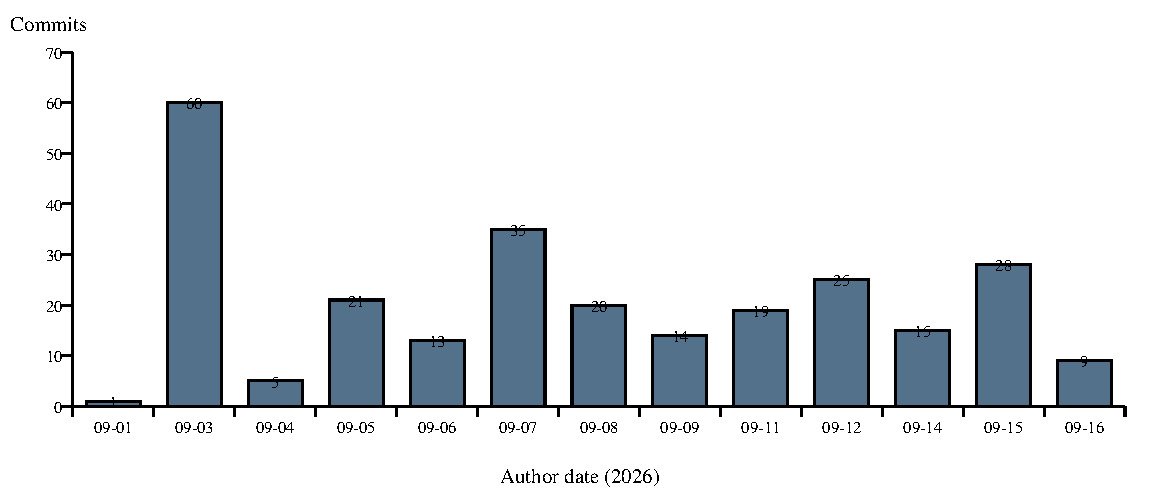
\includegraphics[width=.98\linewidth]{figures/report/git-daily.pdf}\caption{全分支去重后的每日提交数量}\end{figure}
GitHub Insights 页面提供了 Pull Request、作者和分支活动的界面化概览，但平台显示会受到统计范围、默认分支和账号身份的影响。因此，图中数字只作为平台快照，与本节按全部远端分支去重、归并作者身份后的统计结果并列说明，不用来替代前述统计口径。
\begin{figure}[H]
  \centering
  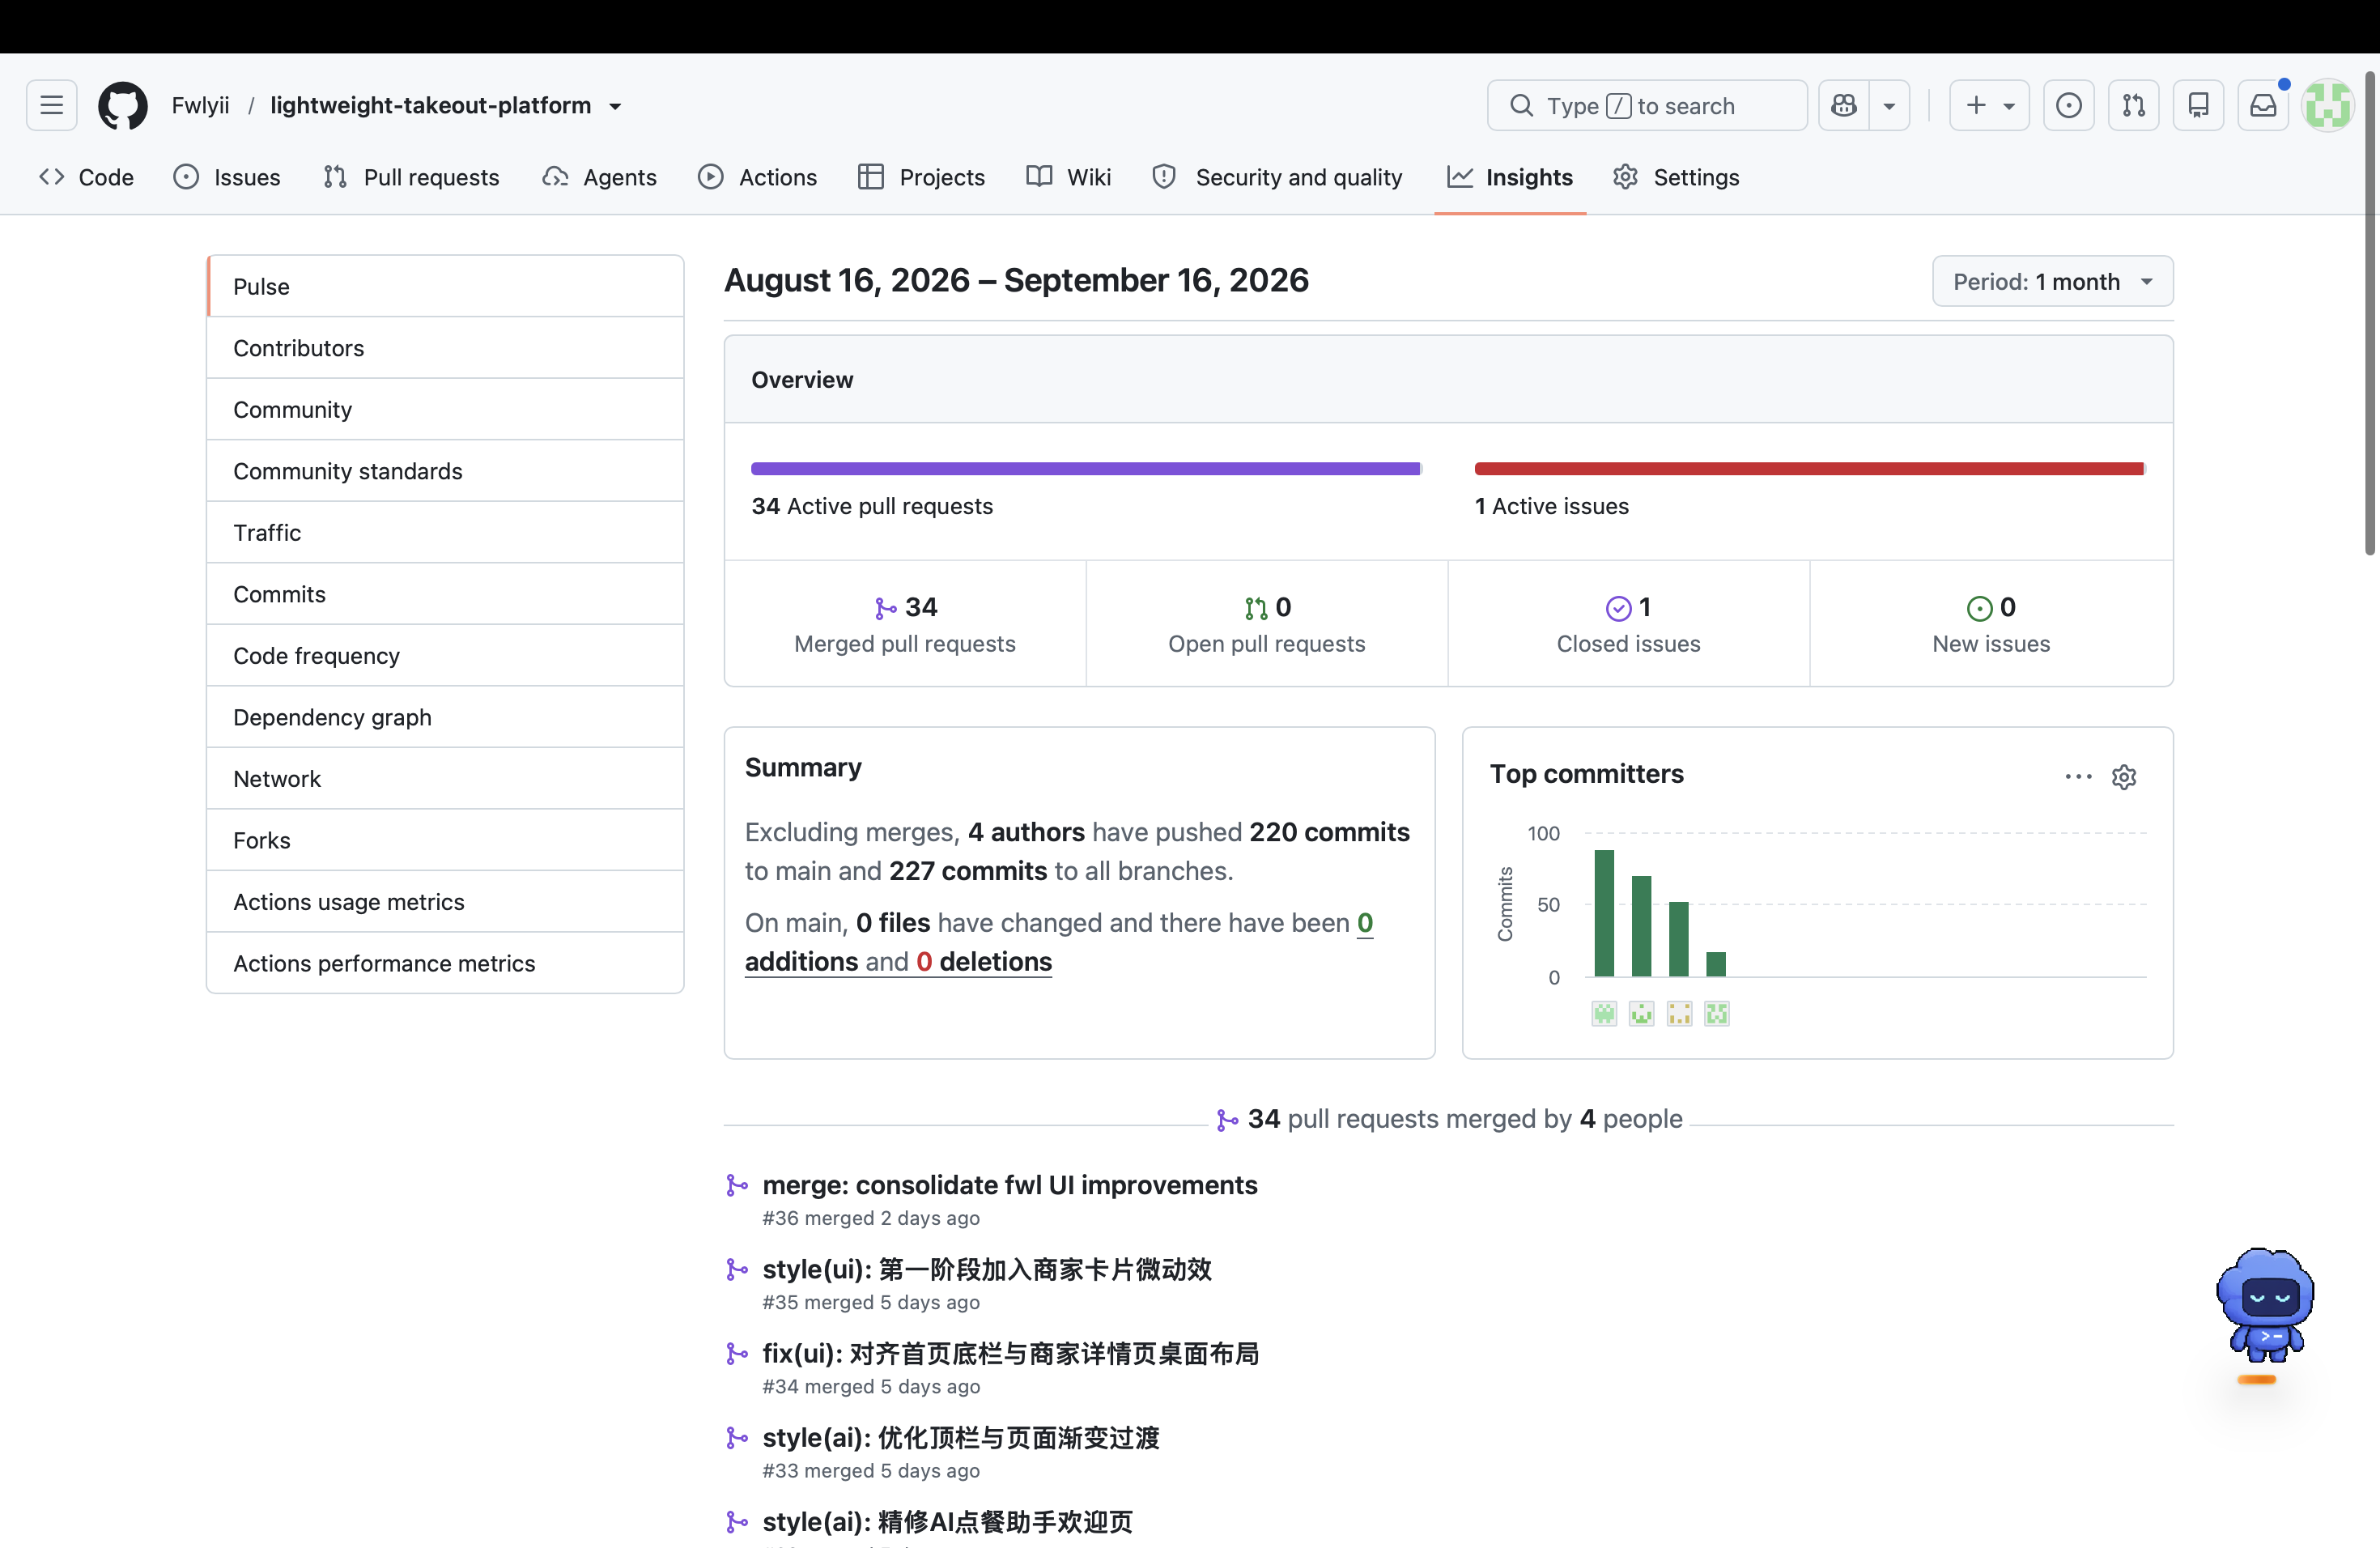
\includegraphics[width=.94\linewidth]{figures/report/process/github-summary.png}
  \caption{GitHub Insights 中的协作活动概览}
  \label{fig:process-github-summary}
\end{figure}
